\chapter{Discussion}\label{chap:discussion}



This chapter will discuss the obtained results, the used methodology, the validity and the reliability of the experiments, adapting the structure proposed by \textcite{luckert2016using}. Section \ref{sec:results-interpretation} will look into the results, describing what has been achieved, as well as indicate the main problems concerning the experiments. Section \ref{sec:method-reflection} will reflect on the research task and discuss whether the right method was chosen to solve the given task. Finally, Section \ref{sec:results-reliability} discusses the validity of the datasets that were used and the overall experiment setup. Based on these validity remarks, this chapter will clarify the reliability of the experiments' results. Therefore, the following questions will be tackled:
\begin{itemize}
    \item What conclusions can be taken from the presented results?
    \item Was the chosen method appropriate for the task?
    \item What benefits and shortcomings have been identified related to the presented work?
    \item What is the validity and reliability of the used data sets and the presented results?
\end{itemize}


\section{Results Interpretation}\label{sec:results-interpretation}

 The following sections present the results for the object-focused agents and environment-focused agents. Mixed-focus agents that explore both octrees and objects are discussed further below in Section \ref{chap5:mixed-focused}. The results are presented from two perspectives: whether the agents have knowledge of voxels or octrees. These perspectives allocate the results according to the research question they answer to. 
 Voxel knowledge is provided when voxel elements are visible in the grid sensor view to the agent, octree knowledge is provided through octree node observations, pigeon observations or observations of the lingering metric.
 
    \subsection{Object Exploration with Knowledge of Voxels} 
        The best object exploration results for this type of agents were achieved by the runs that had a \textit{sparse high voxel reward function}. %among all object-focused agents
        Concretely, \textit{run63+100-nospeed-nolinger} performed the best from the object-focused agents with an average of 1.73 total objects scanned per episode and a standard deviation of 0.17. Close in performance was \textit{run63+100-nospeed}. These two runs prove that an agent that can focus on the scanning of voxels without the distraction of other reward functions achieves the best performance. On this note, even though \textit{run63++025} had the influence of the minimum speed penalty and the lingering penalty, its performance was almost as high as the aforementioned runs. This indicates that it did not have the pressure to change its behavior abruptly when it came into contact with voxels, given that only provided a smaller (25\%) reward.
        An additional point of interest is that some agents do not finish scanning objects, which goes along the lines of the pressure the agent has from these movement penalties. 
        Moreover, the mechanism to reduce the minimum speed penalty and the lingering penalty, if voxels were found in the agent's field of vision (FOV), did not provide the expected performance in \textit{run63++075}, nor \textit{run63++100}.
        An idea is to test the change in performance with an added reward for actually finishing a full scan of an object. This would motivate the agent to finish an object before moving to another one. However, the training setup would sometimes allocate objects within a 10 meter range from each other. The agent would then see both objects and choose to first scan the sides it sees and then the rest of the objects. A possible alternative would be to reward the agent for moving at a slower speed when voxels are in the agent's FOV.
       

    
    
        % were under the pressure of a, perform better at exploration
        On a separate note, the best runs for this section visit more nodes in the environment than their counterparts that included a minimum speed penalty, as shown in Table \ref{tab:results-RQ1-explorative-performance}, even with the \textit{in-field-of-vision} mechanism: they visited an average of 36-40 octree leaf nodes and perceived an average of 119-131 octree scan points, with an octant setup of 4$m^3$.
        In contrast, \textit{run63++075} and \textit{rurn63++100} were able to scan an average of 0.96 and 0.77 total objects per episode respectively, with a standard deviation of 0.17, and visit an average of 29 leaf nodes and perceived 87-90 scan points. 
        These results points towards the hypothesis that the voxel reward function diverges from reward signal of these penalties and the agent cannot easily balance between these two priorities.  
        These results demonstrate that simpler agents, with less distractions, perform better at scanning the objects they need. 
        
        \begin{figure}[!ht]
        \centering
        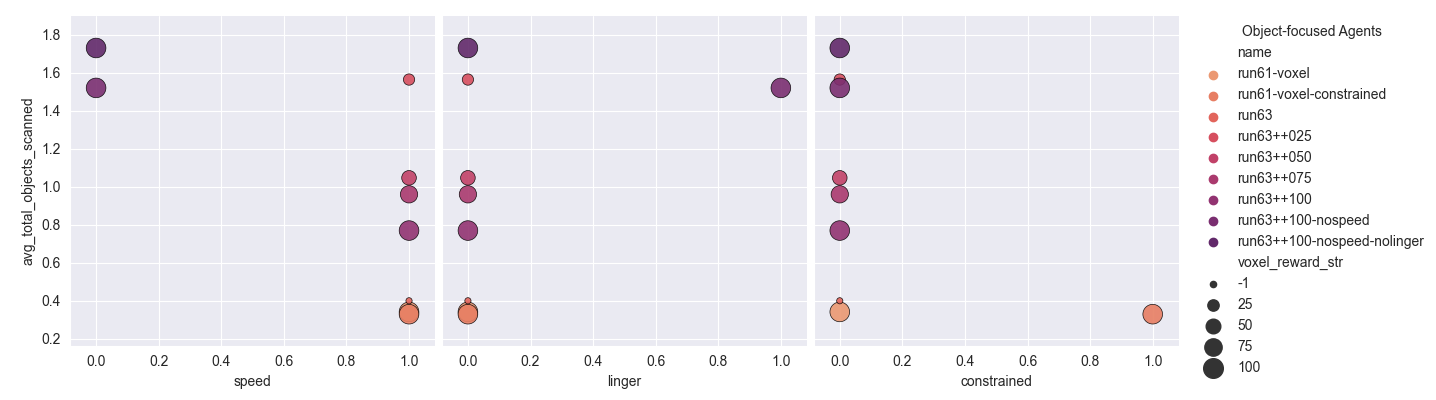
\includegraphics[width=1\textwidth]{images/results_variables_obj.png} 
        \caption{Comparison of the influence of relevant variables on the total amount of objects scanned. The variables for \textit{pigeon} and \textit{pathak} are always set to 1 (active).}
        \label{fig:results_variables_obj}
        \end{figure}
        
        Furthermore, it is important to consider the question of what observations, rewards, and constraints have the greatest impact on the effectiveness of agents in solving particular tasks.
        Based on the performance of the best runs Figure \ref{fig:results_variables_obj} visualizes the influence of the most relevant variables. 
        It shows that agents without the minimum speed requirement perform better when the voxel reward is over 75\% strength, which corresponds to the performance discussed above.
        % Similarly, the agent with a weaker voxel reward could balance with these penalties, at 25\% 
        Furthermore, it shows that the lingering penalty has a smaller influence on the performance of agents, regardless of different strengths of the voxel reward. Finally, the constraint variable confirms that only agents without a normalized voxel reward signal saw sufficient value in the collection of voxels to overcome the penalties of environment. For example, \textit{run61-voxel} only visits 0.5\% of the environment, which, on visual inspection, only spins in circles in the environment.
        
        % Given 6 objects in the scene, the best runs do not explore more than 5\% the environment. This metric is highly dependant on the fact that there are many objects in the scene. Moreover, this metric might also be skewed given collision problems displayed in the visual performance analysis of the drones. More concretely, the best performing agents were very fast at scanning objects, but sometimes they would "crash" against an object and stay still, "stuck" for the rest of an episode.
    
        % This behavior drags the overall average leaf nodes metric down.
        
        % One reason for this behavior could be the training time scale chosen. It has been reported that training at higher time scales can break physics interactions and collisions [ref unity forum]. However, we have chosen a time scale of 20 to avoid such problems.
        
        % However this has proven to be caused by the \textit{collision detection} method set for the \textit{rigid body} of the agent. The initial collision problems were caused by the discrete detection method. Rigidbodies with more active movemement like our drone should prefer to use a variant of the continous detection methods Unity provides. We have chosen to run inference with an speculative collision detection, since our use case does not require fine measurements when the drone collides against obstacles in the scene.
        
        % Something to also consider is the movement algorithm in the agents. It would be interesting to take a closer look at the movement algorithm and even allow the agent to move both left and right at the same time, instead of only left or right. This would provide more freedom in movement according to the situation. 
          
        %   to consider in to consider 
        % \textbf{Mixed-focused agents.} This contrasts, however, with the mixed-focus variants' performance.. 
        % \textit{runs63++025}, which demonstrate that he agent to forget about the minimum speed constraint and focus on scanning the voxels, achieving a similar behavior to \textit{run63++025}. In contrast, 
        % the manual manipulation of features "MAV", with a 0.67 cm error with a standard deviation of 2.46. 
        % The variations of MAV do not show substantial differences, yet they all present an average error higher than 0.5 mm with respect to the ground truth. 
        % The best results among all algorithms for the first research questions were achieved by
        % This contrasts with the other two algorithms, the 
        % An additional subject of interest is the comparison of res
        % Something to consider is that some agents do not finish sc
        % Furthermore, the questions of, which observations and which rewards have the most influence to solve the given problem
        % is an important topic to address. An analysis has been done on the results o
        % This example has been chosen, since it represents the most commonly used attributes for
        
        % Furthermore, as shown in table 4.10, using Google Translate as a candidate, results in
        % substantially higher recall values for automated translation and therefore higher precision
        % values for professional translation
        
        % Assuming, that all Google produced sentences share a characteristi
        
        % The addition of a round-trip translation to be used as 
        
        In summary, the best performing agents achieve an average of 1.73 total objects scanned per episode, visit 36 leaf nodes and are characterized for performing better when removing the minimum speed penalty and, tentatively, the lingering penalty.
    
        % Summarizing, the best achieved results show a classification accuracy of 72:24%, resulting
        % in a gain over a random classifier of 22:24% using Bing Translator as a candidate and
        % Google Translate as a pseudo reference.
    

    \subsection{Object Exploration without Knowledge of Voxels}
        
        This section presents the results for the agents that are receive a voxel reward but are not directly able to see voxels in their grid sensor view.
        
            
        Due to the lack of a sufficient amount of technical documents to train machine learning
        algorithms on a document level, the approach to classify documents into the classes professional
        translation and automated translation consisted of 
        
        To increase the significance of the document-based approach, an additional 19190 manufactured
        documents were ta
        
        An important fact concerning the original document, are the clearly visible differences in
        prediction distributions. 
        
        Another important point of concern, is the question of the percentage share distribution
        of the respective labels. T
        
        It is clearly visible that longer documents deviate less in terms of classification distributions
        than shorter docu
        
        Based on the performance of the best runs Figure \ref{fig:results_variables_obj} visualizes the influence of the most relevant variables.

        % Furthermore, as shown in table 4.10, using Google Translate as a candidate, results in
        % substantially higher recall values for automated translation and therefore higher precision
        % values for professional translation
        
        % Assuming, that all Google produced sentences share a characteristi
        
        % The addition of a round-trip translation to be used as 


        Concluding, although the algorithm classifies every document with one of the two given
        classes, the results cannot always be taken for certain, since the resulting percentage share
        of sentence level classification plays an important role for determining the certainty of
        the classification. The present approach proposes a classification with certainty, if the
        classified document fits into one of the following areas:
         C1, D1 for a classification with professional translation or
         C2, D2 for a classification with automated translation.


    \subsection{Environment Exploration with Knowledge of Octrees}
        
        As mentioned in section 3.3 there was reasonable concern that the amount of existing at-
        tributes using no reference translations was insufficient to create a useful classifier for the
        given problem. 

        The agent with 16 nodes is capable of "covering" much more space 
               
     Based on the performance of the best runs Figure \ref{fig:results_variables_obj} visualizes the influence of the most relevant variables.

            It is size satisfying to see that the pigeon observations provided value in exploration task
        The constraint variable shows that runs with a smaller leaf note size have the highest episode length among the unconstrained runs
        I expected the constrained runs collect the highest episode length

        % Furthermore, as shown in table 4.10, using Google Translate as a candidate, results in
        % substantially higher recall values for automated translation and therefore higher precision
        % values for professional translation
        
        % Assuming, that all Google produced sentences share a characteristi
        
        % The addition of a round-trip translation to be used as 

        Concluding
    
    \subsection{Environment Exploration without Knowledge of Octrees}
        The results discussed above, were used to create a document-based classification system
        similar to the one discussed in subsection 5.1.2. The results for the original documents are
        shown in table 4.15. The first apparent fact is that in this case,
        
        The evaluation shows an average misclassification rate of 32:81% for the shortest documents,
        25:98% for documents containing ten sentences and an average error of 4% for
        document length 250 before dropping to 0% for larger test files.
        As for Research Question 1, the senten
        
        
        The areas of interest are the same as described in subsection 5.1.2. The deviations in the
        areas of larger documents are due to the comparably small amount of created documents
        for lengths of 1000 s

    \subsection{Mixed-focused Exploration} \label{chap5:mixed-focused}
    
            mention using pathak on our models

    \subsection{Comparison of the two Research Questions}

        Concerning the setup of the two research questions, research question 1 was a more
        straight forward task. Allowing the use of reference translations made the creation of
        a valid attribute base easier and the results were more promising in the first optimization
        runs. In contrast to that, the second research question created the problem of having to
        solve a document quality problem without access to semantics of the document, since the
        use of reference translations was not allowed. The addition o
        
        
        Furthermore, the misclassification rate is clearly higher 
        
        
        The figure above shows that misclassifications are strictly lower for every d
        
        
        To further examine the performance between the two systems, it is important to look at
        the percentage share of the different distributions rel
        
        Based on the performance of the best runs Figure \ref{} visualizes the influence of the most relevant variables.
        It is interesting to see that intrinsic curiosity from Pathak's method \cite{pathak2017curiosity} did not provide much value in the expiration task.
        
        
        Concluding, the results of the experiments confirmed the expectations with research question
        1 being easier to solve using classification techniques, than research question 2, due
        to higher overall and averaged accuracies on a sentence level, smaller misclassification
        rates and more certain classifications for all sizes of documents.


    \subsection{Evaluation Framework}

        The proposed framework uses the results of the classification system described in sub-
        section 5.1.1 and therefore assumes that knowledge of the original document is available.
        The framework works on a sentence l
        
        
        
        Additionally, a weighted mistake count is added as additional context information. These
        three attributes (a boolean value for the c
        
        
        The mistake count had more influence on the sentence quality than the classification system,
        resulting in most sentences with a mista
        
        
        Concerning figure 5.6, it is clearly observable that Category 1 and 3 are the most frequent
        classes, which is due to them c
        
        
        It is clearly visible that the professionally translated documents are rated higher than the
        respective automated documents. The reason for the professional documents being rated
        with an average score of 2:00 is 
        
        general interpretation

        Our method performs surprisingly well in a,b,c
        
        the model is robust to hyperparamter tuning, it is shown in the following comparisons under different setups 
        the hyperparemeters tuned were

    
    % \subsection{Small Environment Performance}
    %     From the results of Section \ref{chap-4:small-env-results}, we observe two conclusions:
    %     \begin{itemize}
    %         \item Voxel-curiosity conclusion: The runs that perform the best are run 63 and 68, which are capable of seeing voxels and have no other distractions in terms of training. Interestingly,  Run65 (object detector agent) has shown significant improvements when the minimum speed constraint was removed. We conclude that having sparse and focused reward functions (voxels scanned) tend to a better learning (performing agent) in contrast to denser reward functions. Also in terms of rewards we see that the higher the voxel reward the more attention the agent gives to the collection of voxels, which is expected.


        
    %       \item Octree-exploration conclusion: The results in this run are quite clear: run62 (octree-only agent) is on the lead, since he does not have to split his attention to other tasks other than the discovery of the area. Accordingly, given the small area of 16 $m^2$, it is no surprise that most other runs perform similarly with an average reward of 0.04, since there is not much to be explored in this scene and the goal is only a few steps away from the agent's starting point.
    %     \end{itemize}
        
        
        % \subsection{PPO vs SAC}
        % We find that PPO can significantly improve sample efficiency while not being sensitive to hyperparameter tuning and also has a smaller variance than SAC. We show a few sample runs and present numerical results on a robot control task and a grid world navigation task. \ref{chap:4:summary} \ref{chap:5:robots}
    
    
    % \subsection{Panoramic Performance}
    
  

\section{Method Reflection}\label{sec:method-reflection}

    The used method, adapted from the work by \cite{luckert2016using}, proved to be appropriate for proposing a solution for the research question given. The structure provided allowed for the setup of different experiments without neglecting the initial goal. From the identification of the goal, through the data description and the specification and proposition of the computer vision approaches, the method proved to efficiently structure the work required to construct a pose estimation algorithm using machine learning.
    
    % \subsection{Discuss Abstraction of the World} 
      the benefit of abstracting the world is the reduction of complexity


    The used KDD process proved to be suitable for finding a solution to the two research
    questions. The standardized procedure allowed for the fle
    
    
    
    To address possible translation system specific characteristics, three different machine
    translation system
    
    -
    - a parallel-agent environment where multiple agents could be trained simoulatenously, relatively straight forward but needs some engineering to load multiple configurations at the same time.
    - clarification on: is this LiDAR behavior? >> leads to noise topic, because its not 100\% worth it now
    - noise in visuals when using a real translation from depth
    - noise in scanner, how does the performance suffer ?
    - simplified words: simplified SLAM and model free navigation.
    
    Using different machine learning algorithms to evaluate the quality of sentences and even
    documents, proves to be effective and the results show the adequacy for the task at hand.
    The most known algorithms wer
    
    
    
    Focusing on the initial document quality evaluation on a sentence level ensured the significance
    of the approach, since the used data set consisted of over 20:000 different sentences
    in contrast to the original 14 doc
    Besides the increased significance, 
    However, the taken approach has a clear shortcoming. 
    
    
    
    
    On a similar note, the results in the small environment show that the longer the agent has to move to achieve a goal, the greater the actual difference in the effectiveness of each method.
    % there is an important difference in the actual performance of each method the longer the agent has to move to reach a goal.
    For example, in situations where the goals are distributed scarcely, the agents that are not motivated to explore choose to stick to a small part of the environment. 
    Others chose to move in circles, minimizing the minimum speed penalty, and to wait for the episode to restart. This means that they depend on the domain randomization to spawn a goal near them. It is important to understand that even though these methods are very effective in scanning voxels of objects in the vicinity, such as \textit{run65-pure} demonstrates after visual inspection. However, this does not result in a policy that can be used in a practical environment.
    Moreover, "too small" environments conceal the subtleties that could distinguish one method from another, since they their performance metrics would not be too far apart. 
    Therefore, in order to properly assess exploration policies, we recommend that agents must face not only various scenarios with obstacles, different heights, shapes, and colors but also larger environments that resemble the real world.
    
    
    
    Combining the environment-focused agents with the object-focused agents allowed the final mixed-focused agents to outperform all other variants in the evaluation framework.
    % \subsection{Applicable Practical Scenarios} % Future
    
    It should be noted that in training, many rendering effects, such as grass and moving clouds, do not execute garbage collection mechanisms in the underlying system. This may result in a stop in training if the environment stops reacting due to a lack of remaining memory.
    This may be a problem within Unity ML Agent's plugin episode reset logic, since this problem is not oberved in the test or demonstration runs.
    Training was therefore carried out with the island presented in Chapter \ref{chap:4}, without any post-processing or special rendering effects.
    This corresponded to an average memory usage of 9GB and a load of 60\% across 8 CPU cores, with 5 parallel training environments and a timescale of 20.
    % Nevertheless, the trained agents were tested and fully functional in the applicable practical scenarios which demonstrated the possibility of transfer learning across environments and preserved the agent's explorative behavior.
    As mentioned before, voxel-curious agents, which were trained on voxelized bikes, showed visual-agnostic behavior in other voxelized objects such as buses and homes.
    This validates the proof of concept that our agents can be helpful in emergency rescue situations for police and firefighter drones, environment analysis in factories, airports, warehouses, in industries for defect analysis and product quality assurance, and more.
    
    Furthermore, part of the further use of the results includes the evaluation of compatibility with other environment platforms, such as OpenAI Gym. 
    Unity ML agency provides an OpenAI Gym wrapper that allows any Unity-developed environment to be loaded into a compatible format. 
    This allows for the use of other algorithms, such as custom neural networks and models from OpenAI Baselines \cite{github-dlr-rm-baselines3}.
    From the point of view of compatibility, Unity ML Agent allows indeed smooth transfer to OpenAI Gym.
    However, the results presented in Section \ref{chap:4:cross-platform-compatibility} do not justify the transfer to OpenAI Gym given the lack of out-of-the-box development functions, such as resuming of experiments, logging with Weights and Biases \cite{wandb2022}, debugging, etc. Even though Unity ML-Agents is limited to a set of trainers like PPO and SAC, it provides increased versatility and plug-and-play integration of attention, memory, curiosity, behavioral cloning, auto-curriculum, and many more. Therefore, we consider the use of Unity ML agents to be more appropriate for reinforcement learning tasks as of 2022. The only limitation of the plugin is that it is not possible to load externally created 3D environments.


    % It is therefore up to the researcher o
    % in some area trying to minimize the minimum some of them trying to minimize the minimum speed requirement
        % Similarly when the object is only a few steps ahead the agent is not able the performance between agents the subtleties of the policies of each agent behavior cannot be distinguished because they all perform similarly

% \subsection{Cross-Scenario Performance}
    % Therefore approach expanded the target group of this master's thesis, where further applicability is possible, such as: police investigations, inspection of fire scenes by firefighter drones, factories, warehouses, airport robots, hospital robots, damage detection and analysis, etc. 
        
    
    % % \subsection{Cross-Platform Compatibility}
    % OpenAI gym showed similar performance to mlagents, but the toolbox that comes with it for 
    % took 80\% of the time invested, since    
    In conclusion, the proposed use of octree for environmental exploration and voxels for object exploration has allowed agents to adapt successfully to new environments, to cover large spaces and to perform better than other proposed baselines. Moreover, the evaluation framework clearly distinguishes the performance of the different types of agents. Unity also demonstrated that it has a comprehensive toolkit for implementing concept demonstrations and reinforcement learning agents. Further work includes parsing voxels in real time, taking into account visual input noise and measuring the real-time performance of our methods.


\section{Reliability}\label{sec:results-reliability}
    This section aims to discuss the validity and reliability of the results shown in section \ref{sec:results-research-question}.
    
    The achieved results by the pose estimation algorithm, specially the adaptations done in contribution based off this work, show better performance than the methods in the market for the cow milking robots. The obtained results show promising a performance for current challenges like detecting two cow teats as one. Once the error in the proposed method is reduced, the proposed pipeline could be connected to a memory system that would keep track of the cow teat positions in cases of obstruction from the suction cups, as discussed in Section \ref{sec:future-work}.
    
    In contrast, a few shortcomings related to the achieved results must be mentioned. First, the RANSAC algorithm analysis was limited to RGB images and should have been expanded to evaluate the information from the depth image and the point cloud. Second, a more photorealistic data set should be generated to show DOPE's prediction capabilities and carry out a proper comparison with the "MAV" algorithm. Third, the search space of the parameters adjusted should be wider and not limited to the ones presented. In conclusion, the "MAV" algorithm answers the research question with success, being able estimate the 3D pose and direction of a cow teat in less than 2 seconds.
    
    
        This final section aims to examine the validity and reliability of the shown results in section
    4.2.
    The achieved results show substantial improvement over a given benchmark on a sentence
    level for both research questions. Recombini
    
    
    In contrast to that, a few shortcomings concerning the presented results have to be mentioned.
    First, the results were supposed to focus on a technical documentation domain
    and therefore no statement can be made concerning the classification of documents not
    belonging to the domain. Second, as noted in section 1.5, only syntactical translation
    aspects are taken into account, which means that the classification of a text as a high
    quality document says nothing about the actual meaning of the translation compared to
    the original document. Third, to further evaluate the classification accuracies, an in-depth
    comparison to related experiments using machine learning algorithms on different domains
    should be done to set the achieved results into the scientific context of machine
    translation evaluation on a more general methodology.
    
    Concerning the proposed evaluation approach, the presented framework has been validated
    using sample-based verifications. However, the system still has to be verified by
    professionally qualified institutions to further validate and possibly adapt the proposed
    evaluation classes. In conclusion, the presented approaches answer both research questions
    with success, being able to classify and evaluate technical documents and their translations.
    





\chapter{Conclusion}\label{chap:conclusion}
\section{Conclusions}\label{sec:conclusions}
    This work answered the following research questions:
    \begin{itemize}
      \item How can an embodied agent increase the overall certainty about an object's characteristics, i.e., how can trajectories around objects of interest be generated to reduce the uncertainty about such objects? 
      \item How can these objects be found in large and unknown environments by the same agent?
    \end{itemize}
   
%   We have implemented an efficient data structure for 3D
% point clouds. All presented algorithms are available under the
% GPL license and can be downloaded. The software contains
% a small viewer application that is capable of processing 1
% billion points while still enabling the user to navigate smoothly
% through the point cloud.
% This paper has further presented novel algorithms for the
% efficient processing of very large point clouds. In addition to
% storing and visualizing 1 billion points on modern hardware,
% we are capable of fast shape detection and scan matching.
% In future work we will continue using our octree for efficient
% 3D point cloud processing, e.g., for globally consistent scan
% registration [2], for automatically deriving semantic information, for dynamic maps, i.e., maps that can handle changes of
% the scene, and for next-best-view planning




This was done by modeling and implementing multiple 3D environments in Unity 3D.
These environments were used to train and test several reinforcement learning agents aimed at exploring both objects and environments.
% These environments were used to train and test multiple reinforcement learning agents that aimed to explore both objects and the environment. 
Firstly, objects were explored through the scanning of the voxels that composed the object in the 3D space. 
Secondly, agents learned to explore the environment through extrinsic rewards of the new octree nodes discovered. The resulting agents were visual agnostic and could adapt to multiple environments. Their explorative behavior can also be adapted to a multitude of further scenarios, from product quality assurance drones to rescue, police and firefighter drones. 
Additionally, data collection of 3D scenes is a clear use case for the explorative behavior of the drone, enabling the creation of thorough point cloud datasets in any kind of environment. Given the problematic of small environments proposed by previous methods, our learning environments were 160$m^2$ wide. Our approach was tested against baselines that answered the research questions without direct knowledge of voxels or octrees, respectively. Furthermore, the testing grounds were inspired by the DARPA subterranean challenge to collect data about the time taken to discovery and how much of the environment was explored. Our results show that our exploration drone could explore 90\% of the 3D environment in 3 minutes, whereas methods without the proposed vision explored only 3\% of the environment and did not have the capabilities of exploring objects directly. 

Accordingly, we provided the Unity code for this thesis work and three Unity environments for further work on this project, benchmarks and reproduction of the results. The Unity assets are subject to copyright and require a license to be downloaded and used. We hope that this line of work reaches many people in the community, as the work by Meta Research (Detic) \ref{}, Plenoxels \ref{} and Unity's recent acquisition of Ziva Dynamics \ref{} continue to lay the path for the future of synthetic data and machine learning.

% https://github.com/facebookresearch/Detic
% https://alexyu.net/plenoxels/
% https://blog.unity.com/news/welcome-ziva-dynamics

% and are visual agnostic . cross-environment perform better than alternative methods
% In the current theses work we successfully proposed an agent behavior for autonomous simulated drones that is capable of exploring environments and the optics in it… It reduces the uncertainty environment through the scanning of oxidized objects and takes into account the level of entropy in the environment to provide an indirect this provides an indirect semantic understanding of the states that the agent is in… This method is a général wiiso to other further used cases such as fire accident emergency drones police accident etc. aura for the data collection steps of other methods that require visual input… With that promising future of synthetic data the concept of simplifying environments to construct more complex behaviors homework should be in line… We also successfully provide unity environment that can be further used for benchmarking and extensive billet extensibility of the environment and more… The containers improvement in the machine learning environment machine learning applications with unity continue to grow as seen in their synthetic humans and we hope that more works can follow the lines that we sat down


%     This was done by constructing a data set, training a segmentation algorithm and estimating the pose of the cow teats from the image and the predicted segementation masks. The images for the data set were collected from an artificial cow at the ZHAW using ROSBags to manually export frames at specific timestamps. The images were subsequently annotated and added to the data set. The model was then trained and tested using the generated data set. The false negatives and false positives indicated that more pictures at specific time stamps and positions with respect to the artificial cow had to be added to the data set, to increase the model's accuracy. Consequently, a pipeline was constructed for the independent deployment of the segmentation network and the pose estimation algorithms. The segmentation network would predict and publish segmentation masks for the pose estimation component to consume them and predict, in conjunction with the input images, the pose estimation of the observed cow teats. The methods tested were RANSAC and a manual manipulation approach "MAV". The latter contributed to two other approaches at the ZHAW for the pose estimation of cow teats. From the methods presented in this work, the best results were by a manual approach "MAV", which had a 0.67 cm error with a standard deviation of 2.46. 
    
%     Additionally, an Unreal Engine 4 project for data set generation was constructed for further research. It contains 5 photorealistic scenes with present parameters for rotations and obstructing objects. Finally, a synthetic data set of cow teats was generated with over 400k images for pose estimation. This dataset was used to train the pose estimation algoritmh DOPE, which unfortunately could not close the reality gap and output predictions from real images.

\section{Where to Go From Here?}\label{sec:future-work}
    This work presents a reinforcement learning setup for agents to explore objects and environments. There are a few possible routes for the extension of this work to improve the performance of the achieved results. 
    First, our model-free approach uses synthetic data which greatly simplifies the problematics of the real world \cite{wang2018look}. 
    Our current Unity setup provides noise-free information about the environment through the grid sensor; this is one of the points we would like to tackle in our future work steps which involves the creation of the voxelized environment from the depths of the unity cameras, bringing our method closer to a production setup.
    Second, the implementation of a dynamic, moving, environment would allow us to evaluate the obstacle avoidance capabilities of our agent and, most importantly, the claim that model free approaches suffer given their simplification of the dynamics of an environment \cite{wang2018look}.
    Third, the usage of our model to collect object data and train an object detector, would allow us to directly compare our approach to Chaplot's work \cite{chaplot2020semantic}. Accordingly, the connection to other semantic sub-modules would also bring our agent closer to production.
    Finally, a number of other improvements would benefit the project such as 1) the evaluation of our mobility algorithms and our F1-metric, 2) hyper-parameter sensitivity tests, 3) analysis of attention and memory modules in the Unity ML-Agents plugin, as well as 4) the implementation of a Unity environment that allows curriculum learning using the provided tools by ML-Agents \cite{github-unity-mlagents-toolkit}.
    
    
    % First, a different segmentation network with a faster prediction time could significantly reduce the overall performance time of the presented approach, leading to almost real-time performance. 
    % Second, a memory system could help in cases of obstruction. 
    % For example, when the suction cups are attached, the system could still remember the position of the cow teats and attempt to reattach in case one of the cups detached on movement. 
    % Third, an active vision system could significantly improve the algorithm's time to obtain precise predictions. An active vision system would control the camera position and movement to collect frames with the least amount of movements, so that the objects in the scene could be remembered and understood more efficiently.
    
    % machine learning and computer vision based approach for the 3D pose and direction estimation of cow teats.
    In conclusion, the presented work extends the related research on this topic by a providing a reinforcement learning approach for the exploration of objects and environments for autonomous navigation and simulated agents.
    
    % Furthermore, a big point in model free approaches is the usage of synthetic data which is noise-free and greatly simplifies the features one would see in a real world environment \cite{wang2018look}. 
    
    % Currently our personal performance metrics are separated into the exploration percentage and the number of objects scanned.
    % We consider it would be useful for future work to develop a performance metric that follows the harmnoy concept F1-score achieves between the recall and precision of classifiers. To this end, our metric would balance the performance between exploration percentage and the number of objects scanned in the environment.
    
    % (START DISCUSSION POINTS GRABBED WHILE WRITING)
    % Finally, given trajectories that incorporate the concept of temporal classification entropy, one can sample images to create a dataset for a semantic detector. 
    
    % the work of Learning 3D Semantic Reconstruction on Octrees inspirees further work to look into octree subdivision based onn initial inherent entropy in each node.: motivate resolution of inherent uncerainty in each node by exploring it and motivate subdivisions such as in vespa2019adaptive


    % \subsection{Further Work bullet points >> to be moved to chap 5/6}
    % Further work:
    % \begin{itemize}
    %     \item The analysis of the sensitivity to hyper-parameter of PPO and SAC variants.
    %     \item collision to objects, maybe a penalty because they get "Stuck" next to an object. penalty keep distance to goal
    %     \item motor on two directions
    %     \item 
    % \end{itemize}
    
    % \subsection{Generalization Scenarios}\label{}
    % \subsection{Semantic Sub-modules}\label{}
    
    
    % SOURCE: TENSORFLOW 3D ARTICLE:
    % discussion future work, add photo of encoder
    % In our recent paper, “DOPS: Learning to Detect 3D Objects and Predict their 3D Shapes”, we describe in detail the single-stage weakly supervised learning algorithm used for object detection in TF 3D. In addition, in a follow up work, we extended the 3D object detection model to leverage temporal information by proposing a sparse LSTM-based multi-frame model. We go on to show that this temporal model outperforms the frame-by-frame approach by 7.5% in the Waymo Open dataset.



% In this work we could show that is it possible to acquire a deep scene understanding from sequential
% data with supervised learning. In a simplified use-case such as the presented one, the system can
% successfully acquire a spatial scene understanding that includes objects, their shape, color and even
% their relationship with other objects. Although it is limited to the type of scenes the system was trained
% on, its versatility exceeds by far current mainstream object recognition systems such as ResNet [6].
% Unlike encoder-decoder-based scene understanding approaches such as [32], we do not need specified
% 3D models for training but only a simple scene description that specifies present objects including their
% positions and the camera poses of the captured images. 

% We could show that our system is capable of
% sequentially integrating information from new frames into the existing scene embedding vector. This
% capability is indeed highly remarkable because it includes the achievement of multiple non-trivial steps:
% 1.The change in camera position relative to the previous frame needs to be evaluated. The system does
% not receive any information about the camera position or rotation in space, but needs to extract this
% information based on the difference between the already perceived and the new input frame.2.This
% extracted transformation of the camera position must be used to transform all remembered object
% positions. Some objects might be occluded by the obstacle or other present objects, and the system is
% not able to perceive these items in the current frame. Nonetheless, it is necessary to transform their
% remembered positions so that the system is able to return the correct position when queried. The
% precision of this process however, would need to be further improved when used for robotic grasping,
% as there is still an average deviation of 0.11 meters (about half the diameter of the object) from the
% ground truth when using the best performing approach.

% While our proposed system does not use separated streams for ventral and dorsal pathways, our information
% aggregation process is inspired by the quicker decaying dorsal memory and the more persistent
% ventral memory. This is represented by learned weights versus aggregated temporary information. This
% architecture seems to work great, especially with respect to the 3 different shortcomings that were the
% focus of this work (see section 1.2). In the following, we discuss how our system overcomes them:
%     % \begin{itemize}
%     %     \item 1 paragraph big: describe what was achieved
%     %     \item 1 paragraph: describe our limitations
%     %     \item describe how we "overcame" the shortcommings: 3 paragraphs
%     %     \item closing remarks
%     % \end{itemize}


% \section{Towards Active Vision}
% Since this work was initially inspired by robotic interaction, we would see it as the next step to combine
% our vision-focused system with grasping approaches. An interesting direction would be to work towards
% solving benchmarks for robotic interaction such as RLBench [59].

% When approaching such tasks, we mainly see two possible paths to take: One relatively simple way
% would be to keep the perception and the grasping system separate and only use the output of the
% presented approach as input for a grasp generation algorithm, such as Dex-Net [60]. This would mean
% that the perception part would identify the target object and then forward its position to the grasp
% planning mechanism which would plan the grasp and pass it to the robotic arm for execution. As
% second option it would be possible that the condensed scene representation produced by our system
% would be beneficial for grasp-generation. We think that a promising approach would be to train two
% streams for grasping. The first stream could create a large number of possible grasps, while the other
% one would rate them with likelihood of success. Of course, the system would first need to learn to
% include the required information in the scene representation, which might be a large leap compared to
% the information currently present within the trained system. However, with the human mind closely
% coupling perception and action as part of the dorsal pathway it seems that such a joint approach could
% work for robotic grasping too.
%     % \begin{itemize}
%     %     \item 1 big paragraph describing how active vision could improve accuracy and object permanence
%     % \end{itemize}
% \section{Where to Go From Here?}
% While the discussed approach successfully solves the tasks set, the system is still far from being a real
% replacement for existing computer vision algorithms in use. On the way to the application of a system
% like ours to solve tasks in the real world, it would be necessary to solve at least some of the following
% challenges:

% Real world data: In order to use an approach like the one presented in a real-world use-case, it would
% above all be necessary to transfer the approach to real data or at least more realistic synthetic data.
% With the goal to jointly improve both scene understanding and active vision, we would inspire future
% research to use real-time data gathering with simulated environments as for example Isaac Sim [61].
% This would allow non-discrete view-positions and thus a potentially better understanding. One aspect
% that still might not be solvable by using synthetic data is the noise of the depth-channel of the RGB-D
% data, which is quite prominent for most consumer class RGB-D-camera.

% More different object classes/shapes: The presented solution uses only 5 primitive shapes with 7
% colors, which most likely does not reflect the conditions of a real world use case. A possible solution
% could be the use of large-scale 3D object data sets as used for Dex-Net [60]. Closely related to more
% diverse objects would be the capability to deal with duplicate objects. This could possibly be solved by
% adding multi-object output to all streams (as demonstrated with the Enumerating stream).

% Motion: In this work, we did not address the topic of motion, which does play a big roll in the real
% world. Environments like conveyor belts would be a domain where a scene understanding system like
% the one presented could prove highly useful. However, an application in such an environment would
% require previous research with dynamic scenes.

% Rotation axis detection: With only primitive objects such as cube, cylinders, etc., we decided not to
% include rotation information for our streams. However, for a large number of use cases it could be very
% useful to obtain the rotation of an object, so we would encourage future work to extend our approach
% to include rotation information.
% Grasping/bounding-box detection: For an actual application of robotic grasping, it would be necessary
% to generate possible grasping positions. We did not address this topic in the course of this work
% but leave the extension of the presented approach with grasping to further research. For more details
% see section 5.3.
%     % \begin{itemize}
%     %     \item describe in 5 small paragraphs 5 different future improvements for the voerall system
%     % \end{itemize}


